\documentclass[aspectratio=169,10pt]{beamer}
\usetheme{Madrid}
\usecolortheme{whale}

\usepackage[utf8]{inputenc}
\usepackage{amsmath,amssymb}
\usepackage{tikz}
\usetikzlibrary{shapes.geometric,arrows.meta,positioning,calc,fit,backgrounds,shadows}
\usepackage{booktabs}
\usepackage{xcolor}

\DeclareUnicodeCharacter{20B9}{\textbf{Rs.~}}

\definecolor{primaryBlue}{RGB}{26, 86, 219}
\definecolor{navyDark}{RGB}{15, 23, 42}
\definecolor{textSecondary}{RGB}{71, 85, 105}
\definecolor{canvasBg}{RGB}{248, 250, 252}
\definecolor{cardWhite}{RGB}{255, 255, 255}
\definecolor{borderSlate}{RGB}{226, 232, 240}
\definecolor{statusRed}{RGB}{220, 38, 38}
\definecolor{statusYellow}{RGB}{217, 119, 6}
\definecolor{statusGreen}{RGB}{16, 185, 129}

\setbeamercolor{palette primary}{bg=primaryBlue,fg=white}
\setbeamercolor{palette secondary}{bg=navyDark,fg=white}
\setbeamercolor{palette tertiary}{bg=borderSlate,fg=navyDark}
\setbeamercolor{title}{bg=primaryBlue,fg=white}
\setbeamercolor{frametitle}{bg=primaryBlue,fg=white}
\setbeamercolor{background canvas}{bg=canvasBg}

\setbeamertemplate{navigation symbols}{}
\setbeamertemplate{footline}{
  \leavevmode%
  \hbox{%
  \begin{beamercolorbox}[wd=.35\paperwidth,ht=2.25ex,dp=1ex,left]{author in head/foot}%
    \hspace*{2ex}\textbf{FraudAlert Sentinel} \textbar\ Indian BFSI SOC
  \end{beamercolorbox}%
  \begin{beamercolorbox}[wd=.45\paperwidth,ht=2.25ex,dp=1ex,center]{title in head/foot}%
    Architecture, Real-Time Streaming \& Heuristic Engine
  \end{beamercolorbox}%
  \begin{beamercolorbox}[wd=.20\paperwidth,ht=2.25ex,dp=1ex,right]{date in head/foot}%
    \insertframenumber{} / \inserttotalframenumber\hspace*{2ex}
  \end{beamercolorbox}}%
  \vskip0pt%
}

\title[\textbf{FraudAlert Sentinel}]{\textbf{FraudAlert Sentinel: Real-Time Fraud Defense SOC}}
\subtitle{Architecture, Real-Time UPI Streaming Engine \& Dynamic Heuristic Pipeline}
\author{\textbf{Zensar Advanced Engineering Team}}
\institute{Indian Banking \& UPI Financial Crime Prevention Initiative}
\date{\today}

\begin{document}

% -----------------------------------------------------------------------------
% Slide 1: Title
% -----------------------------------------------------------------------------
\begin{frame}
  \titlepage
  \begin{center}
    \footnotesize \textcolor{white!80}{\textbf{Engineered for RBI Cyber Security Framework, NPCI Interbank UPI, and PMLA Compliance}}
  \end{center}
\end{frame}

% -----------------------------------------------------------------------------
% Slide 2: Executive Overview
% -----------------------------------------------------------------------------
\begin{frame}{Executive Overview: The Challenge in Indian BFSI}
  \begin{columns}[t]
    \begin{column}{0.48\textwidth}
      \begin{block}{\textbf{The High-Velocity UPI Threat}}
        \begin{itemize}
          \item \textbf{14+ Billion} UPI monthly transactions in India.
          \item Sub-second settlement exploited by:
            \begin{itemize}
              \item Rapid velocity mule account rings
              \item Off-hours illicit wire drains (02:00--05:00 AM)
              \item Offshore crypto hawala \& illegal betting
            \end{itemize}
        \end{itemize}
      \end{block}
      \vspace{0.1em}
      \begin{block}{\textbf{Core System Objectives}}
        \begin{itemize}
          \item \textbf{Sub-second Rule Evaluation} on streaming txns.
          \item \textbf{Dynamic RBI/NPCI Rules} with live sliders.
        \end{itemize}
      \end{block}
    \end{column}

    \begin{column}{0.48\textwidth}
      \begin{exampleblock}{\textbf{Tri-Color Risk Triage Standard}}
        \centering
        \vspace{0.2em}
        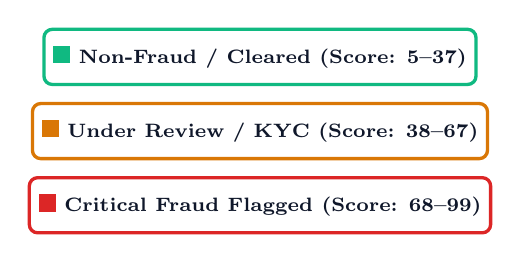
\begin{tikzpicture}
          \node[draw=statusGreen, fill=white, rounded corners=3pt, line width=1.2pt, minimum width=4.8cm, minimum height=0.7cm] (g) {
            \scriptsize \textbf{\textcolor{statusGreen}{\rule{0.22cm}{0.22cm}} \textcolor{navyDark}{Non-Fraud / Cleared (Score: 5--37)}}
          };
          \node[draw=statusYellow, fill=white, rounded corners=3pt, line width=1.2pt, minimum width=4.8cm, minimum height=0.7cm, below=0.2cm of g] (y) {
            \scriptsize \textbf{\textcolor{statusYellow}{\rule{0.22cm}{0.22cm}} \textcolor{navyDark}{Under Review / KYC (Score: 38--67)}}
          };
          \node[draw=statusRed, fill=white, rounded corners=3pt, line width=1.2pt, minimum width=4.8cm, minimum height=0.7cm, below=0.2cm of y] (r) {
            \scriptsize \textbf{\textcolor{statusRed}{\rule{0.22cm}{0.22cm}} \textcolor{navyDark}{Critical Fraud Flagged (Score: 68--99)}}
          };
        \end{tikzpicture}
      \end{exampleblock}
      \vspace{0.1em}
      \begin{alertblock}{\textbf{Key Differentiator}}
        \footnotesize Continuous real-time payload generation (3--5s cadence) evaluated across dynamic weighted thresholds.
      \end{alertblock}
    \end{column}
  \end{columns}
\end{frame}

% -----------------------------------------------------------------------------
% Slide 3: End-to-End System Architecture (Clean Alignment & Spacing)
% -----------------------------------------------------------------------------
\begin{frame}{End-to-End System Architecture}
  \framesubtitle{Four-Tier Real-Time Interbank Processing Pipeline}
  \centering
  \resizebox{0.96\textwidth}{!}{
  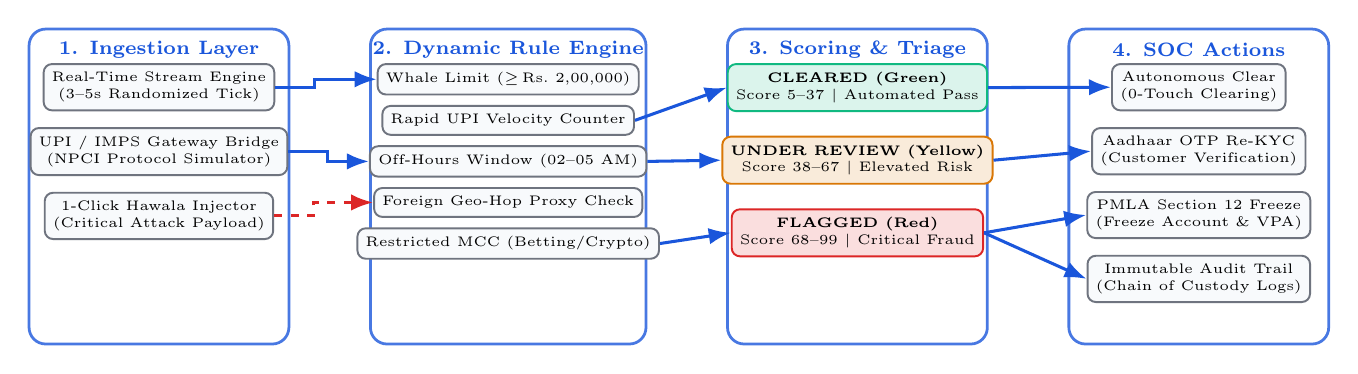
\begin{tikzpicture}[
      layer/.style={draw=primaryBlue!80, fill=cardWhite, rounded corners=6pt, line width=1pt, inner sep=5pt, align=center},
      comp/.style={draw=navyDark!60, fill=canvasBg, rounded corners=3pt, line width=0.7pt, inner sep=3pt, font=\tiny, align=center},
      flow/.style={-Latex, line width=1.1pt, draw=primaryBlue},
      critflow/.style={-Latex, line width=1.1pt, draw=statusRed, dashed}
    ]

    % 1. Ingestion
    \node[layer, minimum width=3.3cm, minimum height=4.0cm] (L1) at (0,0) {};
    \node[font=\bfseries\scriptsize, text=primaryBlue] at ([yshift=-8pt]L1.north) {1. Ingestion Layer};
    \node[comp, below=0.45cm of L1.north] (c1) {Real-Time Stream Engine\\(3--5s Randomized Tick)};
    \node[comp, below=0.20cm of c1] (c2) {UPI / IMPS Gateway Bridge\\(NPCI Protocol Simulator)};
    \node[comp, below=0.20cm of c2] (c3) {1-Click Hawala Injector\\(Critical Attack Payload)};

    % 2. Dynamic Rule Engine
    \node[layer, minimum width=3.5cm, minimum height=4.0cm, right=1.0cm of L1] (L2) {};
    \node[font=\bfseries\scriptsize, text=primaryBlue] at ([yshift=-8pt]L2.north) {2. Dynamic Rule Engine};
    \node[comp, below=0.45cm of L2.north] (r1) {Whale Limit ($\ge$\,Rs.~2,00,000)};
    \node[comp, below=0.12cm of r1] (r2) {Rapid UPI Velocity Counter};
    \node[comp, below=0.12cm of r2] (r3) {Off-Hours Window (02--05 AM)};
    \node[comp, below=0.12cm of r3] (r4) {Foreign Geo-Hop Proxy Check};
    \node[comp, below=0.12cm of r4] (r5) {Restricted MCC (Betting/Crypto)};

    % 3. Scoring & Triage
    \node[layer, minimum width=3.3cm, minimum height=4.0cm, right=1.0cm of L2] (L3) {};
    \node[font=\bfseries\scriptsize, text=primaryBlue] at ([yshift=-8pt]L3.north) {3. Scoring \& Triage};
    \node[comp, fill=statusGreen!15, draw=statusGreen, below=0.45cm of L3.north] (s1) {\textbf{CLEARED (Green)}\\\tiny Score 5--37 \textbar\ Automated Pass};
    \node[comp, fill=statusYellow!15, draw=statusYellow, below=0.30cm of s1] (s2) {\textbf{UNDER REVIEW (Yellow)}\\\tiny Score 38--67 \textbar\ Elevated Risk};
    \node[comp, fill=statusRed!15, draw=statusRed, below=0.30cm of s2] (s3) {\textbf{FLAGGED (Red)}\\\tiny Score 68--99 \textbar\ Critical Fraud};

    % 4. SOC Actions
    \node[layer, minimum width=3.3cm, minimum height=4.0cm, right=1.0cm of L3] (L4) {};
    \node[font=\bfseries\scriptsize, text=primaryBlue] at ([yshift=-8pt]L4.north) {4. SOC Actions};
    \node[comp, below=0.45cm of L4.north] (a1) {Autonomous Clear\\(0-Touch Clearing)};
    \node[comp, below=0.20cm of a1] (a2) {Aadhaar OTP Re-KYC\\(Customer Verification)};
    \node[comp, below=0.20cm of a2] (a3) {PMLA Section 12 Freeze\\(Freeze Account \& VPA)};
    \node[comp, below=0.20cm of a3] (a4) {Immutable Audit Trail\\(Chain of Custody Logs)};

    % Inter-tier Connections
    \draw[flow] (c1.east) -- ++(0.5,0) |- (r1.west);
    \draw[flow] (c2.east) -- ++(0.5,0) |- (r3.west);
    \draw[critflow] (c3.east) -- ++(0.5,0) |- (r4.west);

    \draw[flow] (r2.east) -- (s1.west);
    \draw[flow] (r3.east) -- (s2.west);
    \draw[flow] (r5.east) -- (s3.west);

    \draw[flow] (s1.east) -- (a1.west);
    \draw[flow] (s2.east) -- (a2.west);
    \draw[flow] (s3.east) -- (a3.west);
    \draw[flow] (s3.east) -- (a4.west);
  \end{tikzpicture}
  }
\end{frame}

% -----------------------------------------------------------------------------
% Slide 4: Real-Time Streaming Engine
% -----------------------------------------------------------------------------
\begin{frame}{Real-Time Streaming Engine (`streamService.js`)}
  \framesubtitle{Calibrated Four-Tier Scenario Distribution}
  \begin{columns}[t]
    \begin{column}{0.50\textwidth}
      \begin{block}{\textbf{Streaming Engine Architecture}}
        \begin{itemize}
          \item \textbf{Cadence}: Non-blocking timer fires dynamically every 3000--5000 ms.
          \item \textbf{Ref-Synchronized Ingestion}: Always evaluates against active slider thresholds.
          \item \textbf{Customer Pool}: 10 authentic banking profiles across SBI, HDFC, Axis, ICICI.
          \item \textbf{Telemetry}: Realistic Indian UTRs, IP addresses, VPAs, and timestamps.
        \end{itemize}
      \end{block}
      \vspace{0.2em}
      \begin{alertblock}{\textbf{Zero Alert Fatigue}}
        \footnotesize Stream distribution is calibrated so analysts only receive alerts when transactions legitimately cross risk thresholds.
      \end{alertblock}
    \end{column}

    \begin{column}{0.48\textwidth}
      \begin{exampleblock}{\textbf{Calibrated Scenario Mix}}
        \scriptsize
        \begin{tabular}{llp{3.0cm}}
          \toprule
          \textbf{Tier} & \textbf{Ratio} & \textbf{Representative Merchants} \\
          \par\vspace{0.2em}\dotfill\par

          \textbf{\textcolor{statusGreen}{Good}} & 65\% & Swiggy, Blinkit, Zomato, Uber, IRCTC, D-Mart \\
          \textbf{\textcolor{primaryBlue}{Elevated}} & 15\% & MakeMyTrip, Croma, Mutual Fund SIP, LIC \\
          \textbf{\textcolor{statusYellow}{Review}} & 13\% & Tanishq Jewellery, Apple BKC, Real Estate \\
          \textbf{\textcolor{statusRed}{Attack}} & 7\% & Dubai Crypto Hawala, Casino Goa, Telegram Scam \\
          \bottomrule
        \end{tabular}
      \end{exampleblock}
    \end{column}
  \end{columns}
\end{frame}

% -----------------------------------------------------------------------------
% Slide 5: Dynamic Scoring Model
% -----------------------------------------------------------------------------
\begin{frame}{Dynamic Scoring Model \& Rule Matrix}
  \framesubtitle{Mathematical Formulation of Multi-Factor Risk Scoring}
  \begin{columns}[t]
    \begin{column}{0.50\textwidth}
      \begin{block}{\textbf{Weighted Scoring Formula}}
        \small
        \[
          S_{\text{risk}} = \min\Big(99, \, \max\Big(5, \, S_{\text{noise}} + \sum_{i=1}^5 \delta_i \cdot \widetilde{W}_i + P_{\text{prox}}\Big)\Big)
        \]
        \footnotesize
        \begin{itemize}
          \item $S_{\text{noise}} \sim \mathcal{U}(5, 15)$: Base background noise.
          \item $\widetilde{W}_i = W_i \times (1 \pm \epsilon)$, $\epsilon \in [-0.20, +0.20]$: Jitter.
          \item $P_{\text{prox}}$: Proximity score for near-whale transactions ($60\%\text{--}99\%$ limit).
          \item Scoped Velocity: Only screens recent 30-tx rolling window.
        \end{itemize}
      \end{block}
    \end{column}

    \begin{column}{0.48\textwidth}
      \begin{exampleblock}{\textbf{Active RBI/NPCI Rules Matrix}}
        \scriptsize
        \begin{tabular}{llcc}
          \toprule
          \textbf{Rule ID} & \textbf{Description} & \textbf{Threshold} & \textbf{Weight} \\
          \par\vspace{0.2em}\dotfill\par

          \textbf{RULE-101} & Whale Limit & $\ge$ Rs.~2,00,000 & 45 pts \\
          \textbf{RULE-102} & Rapid Velocity & $\ge$ 4 tx / 30 txns & 35 pts \\
          \textbf{RULE-103} & Off-Hours IST & 02:00--05:00 AM & 25 pts \\
          \textbf{RULE-104} & Hawala Geo-Hop & Offshore Proxy & 50 pts \\
          \textbf{RULE-105} & Restricted MCC & Crypto / Casino & 40 pts \\
          \bottomrule
        \end{tabular}
      \end{exampleblock}
      \vspace{0.2em}
      \begin{alertblock}{\textbf{Diverse Scores Guarantee}}
        \footnotesize Eliminates repetitive scores; scores span organically from 5 to 99 across all transactions.
      \end{alertblock}
    \end{column}
  \end{columns}
\end{frame}

% -----------------------------------------------------------------------------
% Slide 6: Flowchart (Horizontal 2-Row Widescreen Layout — Zero Overflow)
% -----------------------------------------------------------------------------
\begin{frame}{Transaction Lifecycle Flowchart}
  \framesubtitle{Widescreen Horizontal Processing Pipeline (Zero Overflow)}
  \centering
  \resizebox{0.96\textwidth}{!}{
  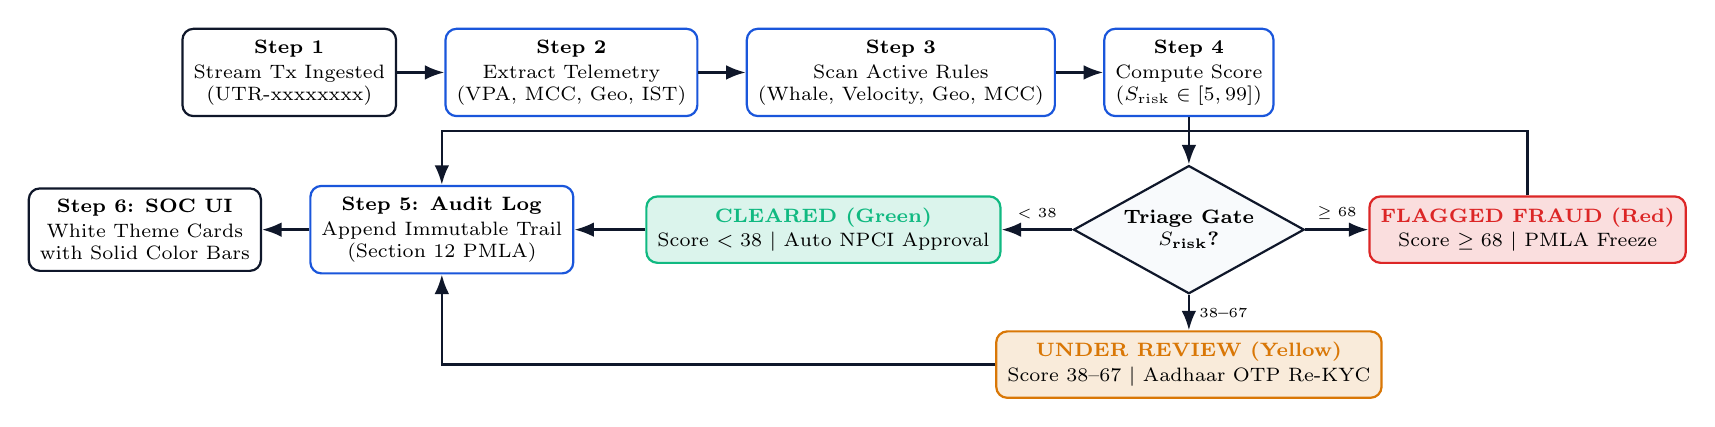
\begin{tikzpicture}[
      box/.style={draw=primaryBlue, fill=cardWhite, rounded corners=4pt, line width=0.8pt, font=\scriptsize, inner sep=4pt, align=center},
      gate/.style={draw=navyDark, fill=canvasBg, diamond, aspect=1.8, line width=0.8pt, font=\scriptsize\bfseries, inner sep=2pt, align=center},
      flow/.style={-Latex, line width=0.9pt, draw=navyDark}
    ]

    % Row 1: Ingestion to Scoring
    \node[box, draw=navyDark] (step1) {\textbf{Step 1}\\[1pt]Stream Tx Ingested\\(UTR-xxxxxxxx)};
    \node[box, right=0.6cm of step1] (step2) {\textbf{Step 2}\\[1pt]Extract Telemetry\\(VPA, MCC, Geo, IST)};
    \node[box, right=0.6cm of step2] (step3) {\textbf{Step 3}\\[1pt]Scan Active Rules\\(Whale, Velocity, Geo, MCC)};
    \node[box, right=0.6cm of step3] (step4) {\textbf{Step 4}\\[1pt]Compute Score\\($S_{\text{risk}} \in [5, 99]$)};

    % Decision Gate
    \node[gate, below=0.6cm of step4] (gate) {Triage Gate\\$S_{\text{risk}}$?};

    % Branch Outcomes
    \node[box, draw=statusGreen, fill=statusGreen!15, left=0.9cm of gate] (bGreen) {
      \textbf{\textcolor{statusGreen}{CLEARED (Green)}}\\[1pt]Score $< 38$ \textbar\ Auto NPCI Approval
    };
    \node[box, draw=statusYellow, fill=statusYellow!15, below=0.45cm of gate] (bYellow) {
      \textbf{\textcolor{statusYellow}{UNDER REVIEW (Yellow)}}\\[1pt]Score $38\text{--}67$ \textbar\ Aadhaar OTP Re-KYC
    };
    \node[box, draw=statusRed, fill=statusRed!15, right=0.8cm of gate] (bRed) {
      \textbf{\textcolor{statusRed}{FLAGGED FRAUD (Red)}}\\[1pt]Score $\ge 68$ \textbar\ PMLA Freeze
    };

    % Bottom Convergence
    \node[box, left=0.9cm of bGreen] (audit) {\textbf{Step 5: Audit Log}\\[1pt]Append Immutable Trail\\(Section 12 PMLA)};
    \node[box, draw=navyDark, left=0.6cm of audit] (ui) {\textbf{Step 6: SOC UI}\\[1pt]White Theme Cards\\with Solid Color Bars};

    % Routing Flows
    \draw[flow] (step1) -- (step2);
    \draw[flow] (step2) -- (step3);
    \draw[flow] (step3) -- (step4);
    \draw[flow] (step4) -- (gate);

    \draw[flow] (gate) -- node[above, font=\tiny\bfseries]{$< 38$} (bGreen);
    \draw[flow] (gate) -- node[right, font=\tiny\bfseries]{$38\text{--}67$} (bYellow);
    \draw[flow] (gate) -- node[above, font=\tiny\bfseries]{$\ge 68$} (bRed);

    \draw[flow] (bGreen) -- (audit);
    \draw[flow] (bYellow) -| (audit);
    \draw[flow] (bRed) |- ++(0,1.25) -| (audit);
    \draw[flow] (audit) -- (ui);
  \end{tikzpicture}
  }
\end{frame}

% -----------------------------------------------------------------------------
% Slide 7: Real-World Scenario Examples (Simple, Clear & Explainable)
% -----------------------------------------------------------------------------
\begin{frame}{Operational Scenarios: Live Screening Examples}
  \framesubtitle{Three Concrete Case Studies Illustrating Dynamic Evaluation}
  \begin{columns}[t]
    % Case 1: Everyday Green
    \begin{column}{0.32\textwidth}
      \begin{exampleblock}{\textbf{Scenario A: Verified Spend}}
        \scriptsize
        \textbf{Merchant}: Swiggy / Blinkit\\
        \textbf{Amount}: Rs.~480 (UPI Instant)\\
        \textbf{Channel}: Mobile UPI PIN\\
        \textbf{Time}: 01:15 PM IST (Daytime)\\
        \textbf{Geo-IP}: Mumbai Domestic\\
        \par\vspace{0.2em}\dotfill\par

        \textbf{Rule Scan}:
        \begin{itemize}
          \tiny
          \item Whale Limit: \textcolor{statusGreen}{\textbf{PASS}}
          \item Velocity Counter: \textcolor{statusGreen}{\textbf{PASS}}
          \item Off-Hours Window: \textcolor{statusGreen}{\textbf{PASS}}
          \item Geo-Hop Proxy: \textcolor{statusGreen}{\textbf{PASS}}
        \end{itemize}
        \par\vspace{0.2em}\dotfill\par

        \textbf{Score}: \textbf{9\,/\,100} (Noise Only)\\
        \textbf{Action}: \textcolor{statusGreen}{\textbf{CLEARED (Green)}}\\[1pt]
        \tiny Zero-friction instant clearance.
      \end{exampleblock}
    \end{column}

    % Case 2: Suspicious Yellow
    \begin{column}{0.32\textwidth}
      \begin{alertblock}{\textbf{Scenario B: Velocity Smurfing}}
        \scriptsize
        \textbf{Pattern}: Rapid Structuring\\
        \textbf{Amount}: Rs.~49,999 $\times$ 4 txns\\
        \textbf{Channel}: IMPS / UPI Fast\\
        \textbf{Time}: 08:45 PM IST\\
        \textbf{Target}: Personal Wallet\\
        \par\vspace{0.2em}\dotfill\par

        \textbf{Rule Scan}:
        \begin{itemize}
          \tiny
          \item Whale Limit: \textcolor{statusGreen}{\textbf{PASS}} ($<$\,Rs.~2L)
          \item Near-Whale Prox: \textcolor{statusYellow}{\textbf{BUMP}} (+12 pts)
          \item Velocity Window: \textcolor{statusYellow}{\textbf{TRIPPED}} (+35 pts)
          \item Customer: 3-month account
        \end{itemize}
        \par\vspace{0.2em}\dotfill\par

        \textbf{Score}: \textbf{52\,/\,100} (Elevated)\\
        \textbf{Action}: \textcolor{statusYellow}{\textbf{UNDER REVIEW (Yellow)}}\\[1pt]
        \tiny Aadhaar OTP Re-KYC dispatched.
      \end{alertblock}
    \end{column}

    % Case 3: Critical Red
    \begin{column}{0.32\textwidth}
      \begin{block}{\textbf{Scenario C: Hawala Drain}}
        \scriptsize
        \textbf{Merchant}: Dubai Crypto Hawala\\
        \textbf{Amount}: Rs.~4,85,000 (Wire)\\
        \textbf{Channel}: RTGS / IMPS Direct\\
        \textbf{Time}: 03:22 AM IST (Off-Hours)\\
        \textbf{Geo-IP}: 194.230.14.88 (Dubai Proxy)\\
        \par\vspace{0.2em}\dotfill\par

        \textbf{Rule Scan}:
        \begin{itemize}
          \tiny
          \item Whale Limit: \textcolor{statusRed}{\textbf{BREACHED}} (+45 pts)
          \item Off-Hours: \textcolor{statusRed}{\textbf{BREACHED}} (+25 pts)
          \item Geo-Hop Proxy: \textcolor{statusRed}{\textbf{BREACHED}} (+50 pts)
          \item Crypto MCC: \textcolor{statusRed}{\textbf{BREACHED}} (+40 pts)
        \end{itemize}
        \par\vspace{0.2em}\dotfill\par

        \textbf{Score}: \textbf{99\,/\,100} (Critical Threat)\\
        \textbf{Action}: \textcolor{statusRed}{\textbf{FLAGGED FRAUD (Red)}}\\[1pt]
        \tiny Instant PMLA Freeze \& VPA Block.
      \end{block}
    \end{column}
  \end{columns}
\end{frame}

% -----------------------------------------------------------------------------
% Slide 8: UI Design System & Horizontal Status Bar Cards
% -----------------------------------------------------------------------------
\begin{frame}{SOC Analyst Interface}
  \framesubtitle{Enterprise White Theme \& Horizontal Color Bars}
  \begin{columns}[t]
    \begin{column}{0.48\textwidth}
      \begin{block}{\textbf{Stitch Design System Tokens}}
        \begin{itemize}
          \item \textbf{Enterprise White Surface}: \texttt{\#FFFFFF} cards on \texttt{\#F8FAFC} canvas.
          \item \textbf{Solid Horizontal Status Bars}:
          \begin{itemize}
            \item \textcolor{statusRed}{\textbf{Solid Red Bar}}: High-risk mule \& hawala threats.
            \item \textcolor{statusYellow}{\textbf{Solid Yellow Bar}}: High-value review cases.
            \item \textcolor{statusGreen}{\textbf{Solid Green Bar}}: Cleared everyday payments.
          \end{itemize}
          \item \textbf{Dual View Toggle}: Seamlessly switch between \textbf{Horizontal Bar Cards} and \textbf{Dense Table View}.
        \end{itemize}
      \end{block}
    \end{column}

    \begin{column}{0.48\textwidth}
      \begin{block}{\textbf{Forensic Drill-Down Modal}}
        \begin{itemize}
          \item \textbf{Entity Profiling}: Customer VPA, bank tenure, average monthly spend.
          \item \textbf{Chain of Custody}: Detailed history of tripped rules and timestamps.
          \item \textbf{1-Click Enforcement}:
          \begin{itemize}
            \item \textbf{Freeze UPI / VPA}: Direct Section 12 PMLA block.
            \item \textbf{Aadhaar OTP Re-KYC}: Re-authenticate customer via OTP.
            \item \textbf{Dismiss Case}: Audit-justified false positive sign-off.
          \end{itemize}
        \end{itemize}
      \end{block}
    \end{column}
  \end{columns}
\end{frame}

% -----------------------------------------------------------------------------
% Slide 9: Technical Architecture & Stack
% -----------------------------------------------------------------------------
\begin{frame}{Technical Architecture \& Codebase Structure}
  \framesubtitle{Modern Frontend Stack \& In-Memory State Synchronization}
  \begin{columns}[t]
    \begin{column}{0.50\textwidth}
      \begin{block}{\textbf{Core Components Topology}}
        \begin{itemize}
          \item \textbf{\texttt{AppContext.jsx}}: Global state for live transactions, rules, audit logs.
          \item \textbf{\texttt{rulesRef} \& \texttt{transactionsRef}}: Prevent stale closures in async streaming loop.
          \item \textbf{\texttt{streamService.js}}: Randomized 3--5s generator across 4 tiers.
          \item \textbf{\texttt{TransactionTable.jsx}}: Card \& Table rendering with solid color bars.
          \item \textbf{\texttt{CaseReviewModal.jsx}}: Full analyst forensic investigation suite.
        \end{itemize}
      \end{block}
    \end{column}

    \begin{column}{0.48\textwidth}
      \begin{exampleblock}{\textbf{Technology Stack}}
        \scriptsize
        \begin{tabular}{ll}
          \toprule
          \textbf{Layer} & \textbf{Technology} \\
          \par\vspace{0.2em}\dotfill\par

          \textbf{Framework} & React 18, JSX, Functional Hooks \\
          \textbf{Bundler} & Vite Fast Refresh (ESM) \\
          \textbf{State Engine} & React Context + Ref Synchronization \\
          \textbf{Design Tokens} & Stitch White Theme + Vanilla CSS \\
          \textbf{Currency Format} & \texttt{Intl.NumberFormat} (INR Lakhs/Crores) \\
          \textbf{Persistence} & LocalStorage (Isolated Indian BFSI Keys) \\
          \bottomrule
        \end{tabular}
      \end{exampleblock}
    \end{column}
  \end{columns}
\end{frame}

% -----------------------------------------------------------------------------
% Slide 10: Conclusion & Operational Impact
% -----------------------------------------------------------------------------
\begin{frame}{Operational Impact \& Summary}
  \framesubtitle{Protecting the Next Billion UPI Users}
  \begin{columns}[t]
    \begin{column}{0.50\textwidth}
      \begin{block}{\textbf{Key Operational Outcomes}}
        \begin{itemize}
          \item \textbf{Sub-10ms Screening Latency}: Pre-clearance transaction validation.
          \item \textbf{Zero Alert Fatigue}: Jittered 5--99 risk scoring ensures accurate triage.
          \item \textbf{Zero-Downtime Rule Tuning}: Immediate policy threshold adaptation.
          \item \textbf{PMLA Section 12 Ready}: Tamper-evident immutable audit trails.
        \end{itemize}
      \end{block}
    \end{column}

    \begin{column}{0.48\textwidth}
      \begin{exampleblock}{\textbf{Next Generation Roadmap}}
        \begin{itemize}
          \item Integration with NPCI's UPI Safety Shield API.
          \item ML Graph Neural Networks for multi-hop mule detection.
          \item Automated RBI FIU-IND XML reporting export.
        \end{itemize}
      \end{exampleblock}
    \end{column}
  \end{columns}

  \vspace{1.0em}
  \begin{center}
    {\large \textbf{\textcolor{primaryBlue}{Thank You!}}}\\[0.2em]
    \footnotesize \textbf{FraudAlert Sentinel} \textbar\ Autonomous Real-Time Financial Defense for Indian BFSI
  \end{center}
\end{frame}

\end{document}


